\chapter{Architecture and implementation of the Journal and Stream Processing part}

\section{Architecture}

As presented in the Requirements chapter, the Journal needs to store the events an append-only list. The Journal should also provide a way for stream processors to subscribe 
to the real-time stream of events. Stream processors can subscribe to themselves in a Tree-like structure (see Figure \ref{fig:tree}), and upon the reception of an event can create a substream of events and perform a side-effect.
\\

\subsection{Naive push-only solutions}

A important problem that will model the architecture is the fact that the Journal can have an event stream rate that is superior to its subscribers. More generally,
any parent node (Journal or processor) can have a output stream rate that is superior to one or several of its children. 
Several simple \textit{push} solutions can be applied, but none of them were applicable for our system.

First, any child can just have a in-memory buffer that store the incoming events not yet processed. However, an in-memory buffer has obvious limitations like the danger
of causing an OutOfMemory exception. Moreover, as said in the non functional requirements part, one goal is to limit the RAM consumption of the platform. Thus, this solution is
not applicable.

Another solution can be for a parent node to wait that all its children have processed the current event to send the next one via an ACK mechanism. 
An obvious issue of this approach is that
the slowest child of a parent will slow down the event stream rate for every of its siblings. This is clearly not acceptable for a scalable system with loose coupling 
between components. Moreover, such a solution implies that the failure of a child stops the stream for its siblings, which is clearly unacceptable.

As a reminder, no message loss is a requirements for the platform, so dropping the events if the stream rate is too fast is not an option.
\\

\subsection{Pull-based streaming with event-sourced processors}

One suitable solution is to use a pull-model instead of a push-model. For each received event, a processor processes it to produce a substream, optionally do some
side effects on the substream, and stores this substream in a local journal. Thus, each processor maintains its own event journal, so each processor is \textit{event-sourced}.
This allows each child to maintain a cursor on the journal of its parent pointing on the next event to pull. Thus, children can have totally different pulling and processing speed, they are not coupled to each other. This approach of pull-based stream system with decoupled multi-consumers using cursors comes from Apache Kafka, a distributed messaging system for log processing created at LinkedIn \footfullcite{bib:kafka}. 

A common problem with pull based-system is the polling part. How do children to known when the next event is ready to be pulled? The naive way to do this is to check every X seconds / milliseconds if the parent has a new event in its journal. This can waste a lot of resources when a parent has no new event for a while. The solution brought by Kafka is to 
perform long-polling: when the child's cursor go the next event, either it pulls the next event if it exists or it blocks until a new event comes in to pull it. Thus, children does not have to pull periodically to know if there is a new event.

However, the term "blocks" does not really get along well with our reactive non-blocking architecture. We therefore have to find a way to implement long-polling without blocking
threads. To do that, we will use a new functional programming abstraction that comes with Futures: Promises. Mixing Futures, Iteratees and Promises, we will be able to implement
an asynchronous non-blocking long-polling system (more details in the Implementation section \ref{sec:streamimplementation}).

Both the Journal and the local journals of processors are persistent using MongoDB. MongoDB is a document-oriented NoSQL database \footfullcite{bib:mongodb} that stores BSON documents (a binary representation of JSON). The format of stored event is a BSON-serialized version of ZEvents (see Listing \ref{lst:zevent}). It contains an id, the name of the resource (for example \verb|/resourceType1/id4|), the user that inserted the event in the Journal, the insertion date, the type of event and the body (data) of the event in a JSON object. To model a journal, we just use a MongoDB collection where we only insert new documents (events). To keep the insertion order of events, an id of type PathId is serialized
into the document. MongoDB provides a built-in id generation mechanism that keep the insertion order, but the fact of ensuring message ordering of substream across processors implies to create a more sophisticated id generation mechanism. This will be explained thoroughly in section \ref{sec:substreamproblem}.
\\

Thus, each event produced by a processor goes into its MongoDB local journal, and children pull events (one by one or by bulk) according to their position in their parent
local journal. If one or several of them is "up-to-date" with the last event of its parent, a long-polling mechanism allows to prevent them to waste resources periodically pulling their parent.

However, this mechanism can be improved. For example, if a parent processor knows that one of its children is "up-to-date", it can directly send him the next event without
passing by the persistent storage to improve efficiency. This approach is described in the next section.

\subsection{Fault-tolerant persistent processors with exactly-once side-effect semantic using Path Ids}
\label{sec:substreamproblem}

Of course, a persistent storage on MongoDB allows fault-tolerance in case of a processor crashes and restarts. When a processor restarts, it checks in MongoDB what was the
last id of the event it successfully processed before crashing, and ask its parent for the next event after this id (it \textit{replays} the stream from where it crashed).
However, if a processor crashes \textit{during} the processing of an event, how to know if it has successfully and entirely processed this event? What it means to process "entirely" an incoming event?
\\

First, we differentiate the \textbf{process} method and the \textbf{performAtomicSideEffect} method in a processor. As stated in the Requirement chapter, the process method 
takes one event and produces a substream of events from it. Its signature is \verb|process(event: I): Enumerator[O]| where I is the type of input events and O the type
of out events. As we saw in the previous parts, an Enumerator is a functional abstraction for a non-blocking stream producer. The function implementing the process interface
should be pure, i.e should not have any side-effect. More precisely, it can have side-effects, but the call semantic of this function is \textit{at-least-once} for each 
event, meaning that the same side-effect can be called several times. Thus, it is ok to have idempotent side-effects. However, for side-effects that are non-idempotent and
thus requires \textit{exactly-once} semantic, one can use the performAtomicSideEffect method whose signature is \verb|performAtomicSideEffect(event: O): Future[Unit]|.
The function is called for each output event of the created sub-stream and is guaranteed to be called exactly-once for each output event even in cases of failures. The
Future[Unit] returns type is a Future returning nothing (normal for a side-effect). The difference of returning Future[Unit] instead of simply returning Unit is that a side-effect
can be asynchronous but returning a Future of nothing allows us to known when this side-effect is finished. This enables to ensure sequentiality of side-effect (the side-effect
of the out event 1 in the substream will be finished when the side-effect of out event 2 begins).

With these two functions, fault-tolerance is handled in a clear manner. process is an user-defined function that is the logic of the processor: how to derive one event to a substream of derived events. As a pure function, it is not a problem if it is called several times for the same input. performAtomicSideEffect is then used on each event to
save the event to a local journal. This operation must me \textit{atomic}. Thus, if a processor crashes, when it recovers it just take the last out event id processed LastID and its parent for the event that generated the substream containing this out event. The parent re-sends this event which is put again in the process method (at-least-once call semantic).
This process method re-creates the substream, and a filter is put on the substream to take only the out events that are \textit{after} the original LastID ouptut event. This
filtered substream is then given to the performAtomicSideEffect method that goes on saving events as usual.
Thus, we have ensured no message loss, no message duplication and guaranteed message ordering in cases of processor crashes. It is easy to see why the "insert in journal" operation in performAtomicSideEffect needs to be atomic: if it is not (say it has 2 steps), if the processor fails between step 1 and step 2, we are in a position where
we don't know if the current out event has been inserted or not where the processor recover. 

This atomicity leads to a potential problem: if we already use the performAtomicSideEffect for inserting output events in the journal, there is no room left for an arbitrary side-effect that can be defined by the user of the library. This is why we define two kinds of processors: \textit{persistent} processors where the performAtomicSideEffect is already implemented to insert output events in a local journal (the type of processor described in this section), and \textit{side-effect} processors that allows to define
an arbitrary atomic side-effect. Side-effect processors will be described in details in section \ref{sec:sideeffectproc}.

Thus, for a persistent processor, the fact that an input event has been "entirely" processed means that all of the events in the substream it has generated are inserted in the local journal.
\\

One key operation that has not been explained is how to know which input event has generated a particular output event generated in a substream. This is a complex task for which the notion of Path Ids has been created.

\subsubsection{Auto generation of tree-like Ids: Path Ids}

The generation of events across the tree of processors can be seen itself as a event tree. For example, when event 1 comes from the Journal and enter in the first
processor, event 1 can generate a substream of events (say event 1-1, event 1-2 and event 1-3). Then, a child processor that generate a 2-event substream
will generate event 1-1-1, event 1-1-2, event 1-2-1, event 1-2-2, event 1-3-1 and event 1-3-2 (see Figure \ref{fig:treepathid}).

\begin{figure}[h]
  \begin{center} 
    \makebox[\textwidth]{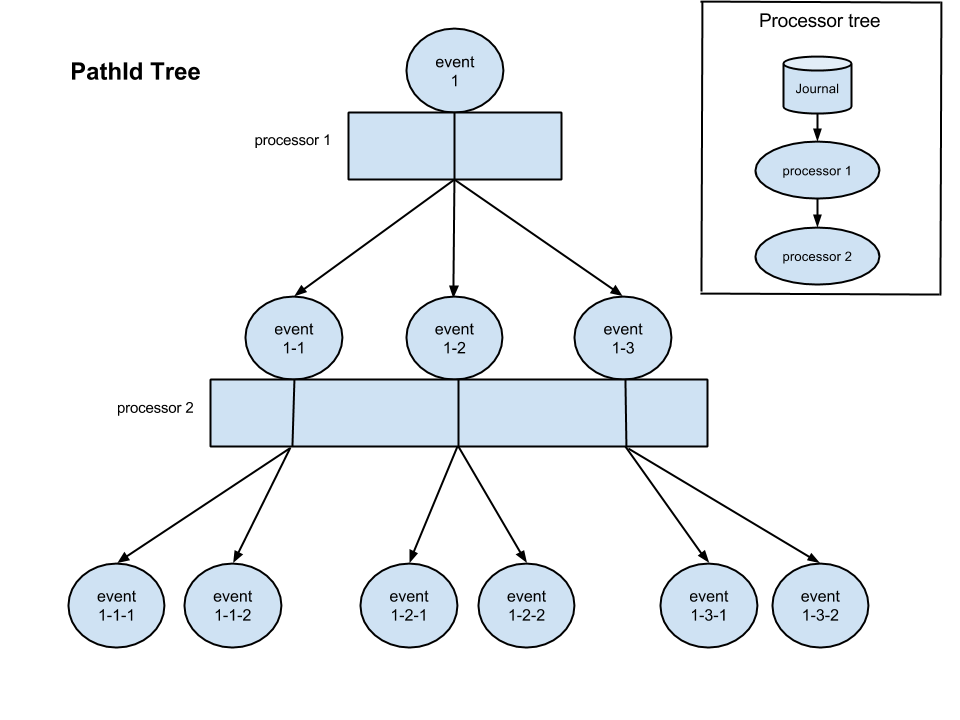
\includegraphics[width=1.0\textwidth]{img/id_tree.png}}
    \caption{A generational tree of PathIds}
    \label{fig:treepathid}
  \end{center}
\end{figure}

We see that the generation of events has a tree-shape, and each event can be characterized by a path in this tree (for example, 1-2-1). This idea of PathId is to
auto-generate these path ids when event passes through processors so that it is possible to re-climb the tree given a particular event.

Concerning fault-tolerance, a child processor that recovers after a crash can check its last PathId, remove the last node of it and send the new PathId to its parent. Then, the parent send him the event that it re-processed (re-creating the substream), and thanks to the number of the last node the child can know from where in the substream it crashed. The idea of id generation to be able to retrieve from a child event the parent event comes from Apache Storm, a distributed and fault-tolerant real-time computation framework \footfullcite{bib:storm}.

The implementation part will explains in more details of these PathIds are serialized and deserialized in MongoDB.

The ability of re-climbing the generational tree is also very useful for side-effect stream processors described in next section.

\subsection{Side-effect stream processors}
\label{sec:sideeffectproc}

Persistent processors use their performAtomicSideEffect method to insert the generated events in their local journal. We saw that a persistent processor can only do one
atomic side-effect per generated event in order to guarantee exactly-once side-effect semantic even in cases of failure. So it is not possible to update
an incremental custom view on arbitrary data contained in the event for example.

Thus, we define another type of processor where one can implement an arbitrary side-effect in the performAtomicSideEffect method: side-effect processor. The contract
for this side-effect is that it is atomic if one wants to have the exactly-once side-effect semantic, and moreover the side-effect of event of PathId N should store
this PathId somewhere to be able to retrieve it when it recovers. Note that this is not the same than inserting the event in a journal as in persistent processors:
here we only need to store the PathId, not the entire event. Upon a recover, a method getLastProcessedEventId of signature 
\verb|getLastProcessedEventId(): Future[PathId]| is able to retrieve the last PathId processed to initiate the recover mechanism explained in the previous section.
\\

Thus, side-effect processors does not store the whole list of events but only the last PathId processed. It brings a problem if a child of a side-effect processor
wants to replay past events because it is slow or because it crashed. To solve this, side-effect processors ask their own parent to replay the stream of events.
This is a recursive call until the nearest parent processor that is persistent which is the tree root (Journal) in the worst case. 

Moreover, each intermediate side-effect processor in this recursive call must take care of sending only the minimal amount of messages in substreams. Indeed,
as we re-climb the generational PathId tree, each event send by a parent is put in the process method that generates the substream. We must generally just send
events from this substream from a certain event because all events generated from previous events of the substream has already been processed by children. 

Figure \ref{fig:sideeffectreclimb} illustrates this mechanism. If side-effect processor 2 fails just after the processing of event 1-2-1, TODO
\\

In the end, side-effect processors allows to define an arbitrary side-effect (with some constraints), allows to save disk space because it does not maintain
a local journal, but it implies that event streams replays take longer because a side-effect processor cannot replay the stream itself, it has to ask to its parent.

TODO: side-effect needs to save last process id
TODO: no need to save all events, but replayabilty takes longer

=> at least once for processing, different than side-effect !


\subsection{Adaptive push-pull streaming with back-pressure}

Asynchronous in - out in processors

The pull-based mechanism can be improved to limit the accesses to the local persistent journal.


Optimization: push mode with child states in parent node

explain back-pressure thoroughly, TCP included ! (maybe in its own subsubsection) (see Evernote for bib)

The "ACK" mechanism is at TCP-level in distributed mode -> very efficient !


\subsection{The Journal case: ensuring ordering with non-replayable multiples sources}

Mongo IDS ?

Only in impl part ? no...



\section{Implementation}
\label{sec:streamimplementation}

\subsection{Abstractions choice}

TODO: pas Actors car:
- pas back-pressure auto
- sequentiality of async op pas auto, besoin de stash, in-memory inefficient car remet dans la mailbox a chaque fois...

--> Custom Stream Processor abstraction on top of Iteratees/Futures/Promises !

\subsection{...}

TODO: explains pathid SerDe in Mongo
TODO: explains long-polling promises...

